\section{Results and discussion}
% Structure with subsections
% Use of figures/tables (max. 5)
% General description of the results
\subsection{Differentially Expressed Genes and Network Creation}

Under the chosen thresholds discussed in section \ref{sec:methods-deg}, 908 genes were found to be differentially expressed. Around half (495) are up-regulated, and the remaining 413 are down-regulated. STRING could query 828 of them; using other ID types did not change this. After querying the additional EDS-related genes, the resulting network consists of 847 genes and 6129 connections.

The position of the known EDS genes in the network is, on average, more central than expected by chance based on degree, clustering coefficient, betweenness centrality and closeness centrality, supporting the close relationship between hEDS and other EDS types.

\subsection{Enrichment analysis and clustering}

GO-enrichment is performed on the DEGs to acquire an overview of over-repersented molecular functions, biological processes and cellular components.  

\begin{itemize}
	\item Cellular Component: Nuclosome, collagen-containing extracellular matrix, chromatin, chromosamal region [TODO: dot plot or graph?]
	\item Biological Progress: nucleosome assembly \& organization, protein-DNA assembly \& organization, cell clycle signaling, regulation \& transition, chromosome separation regulation
	\item Molecular function difficult to analyse on large graph, but we see structural constituent of chromatin, protein heterodimerization activity and extracellular matrix structural constituent
\end{itemize}


TODO

\subsubsection{MCODE}
Running MCODE on the created networks finds 3 clusters with more than 15 genes, one with 66 genes and 1953 connections, one with 44 genes and 686 connections and one with 16 genes and 114 connections with the second two clusters containing up-regulated genes only. The two bigger clusters contain no genes known to cause other EDS types. % TODO: interpretation - might those be processes that we see only in hEDS and not in other EDS types? Look at heat in community cluster

\paragraph{MCODE cluster with EDS genes}
The third, smaller cluster, shown in figure \ref{fig:mcode3}, contains mostly up-regulated but also two down-regulated genes. Some do not show a strong differential expression but are genes known to cause other EDS types. In total, the cluster contains eight EDS genes, all having a $|\text{log2FoldChange}| < 0.5$ and nine differentially expressed genes. One of the EDS genes is also one of the two down-regulated genes. All known EDS genes besides ADAMTS2 have a high Closeness Centrality, consistent with the findings of EDS genes being more central in the complete network. COL21A1 shows the strongest differential expression ($\text{log2FoldChange} > 2$), more than twice as high as the other genes while being less central in the cluster.

\begin{figure}[htb!]
	\centering
	\caption*{\textbf{MCODE cluster 3}}
	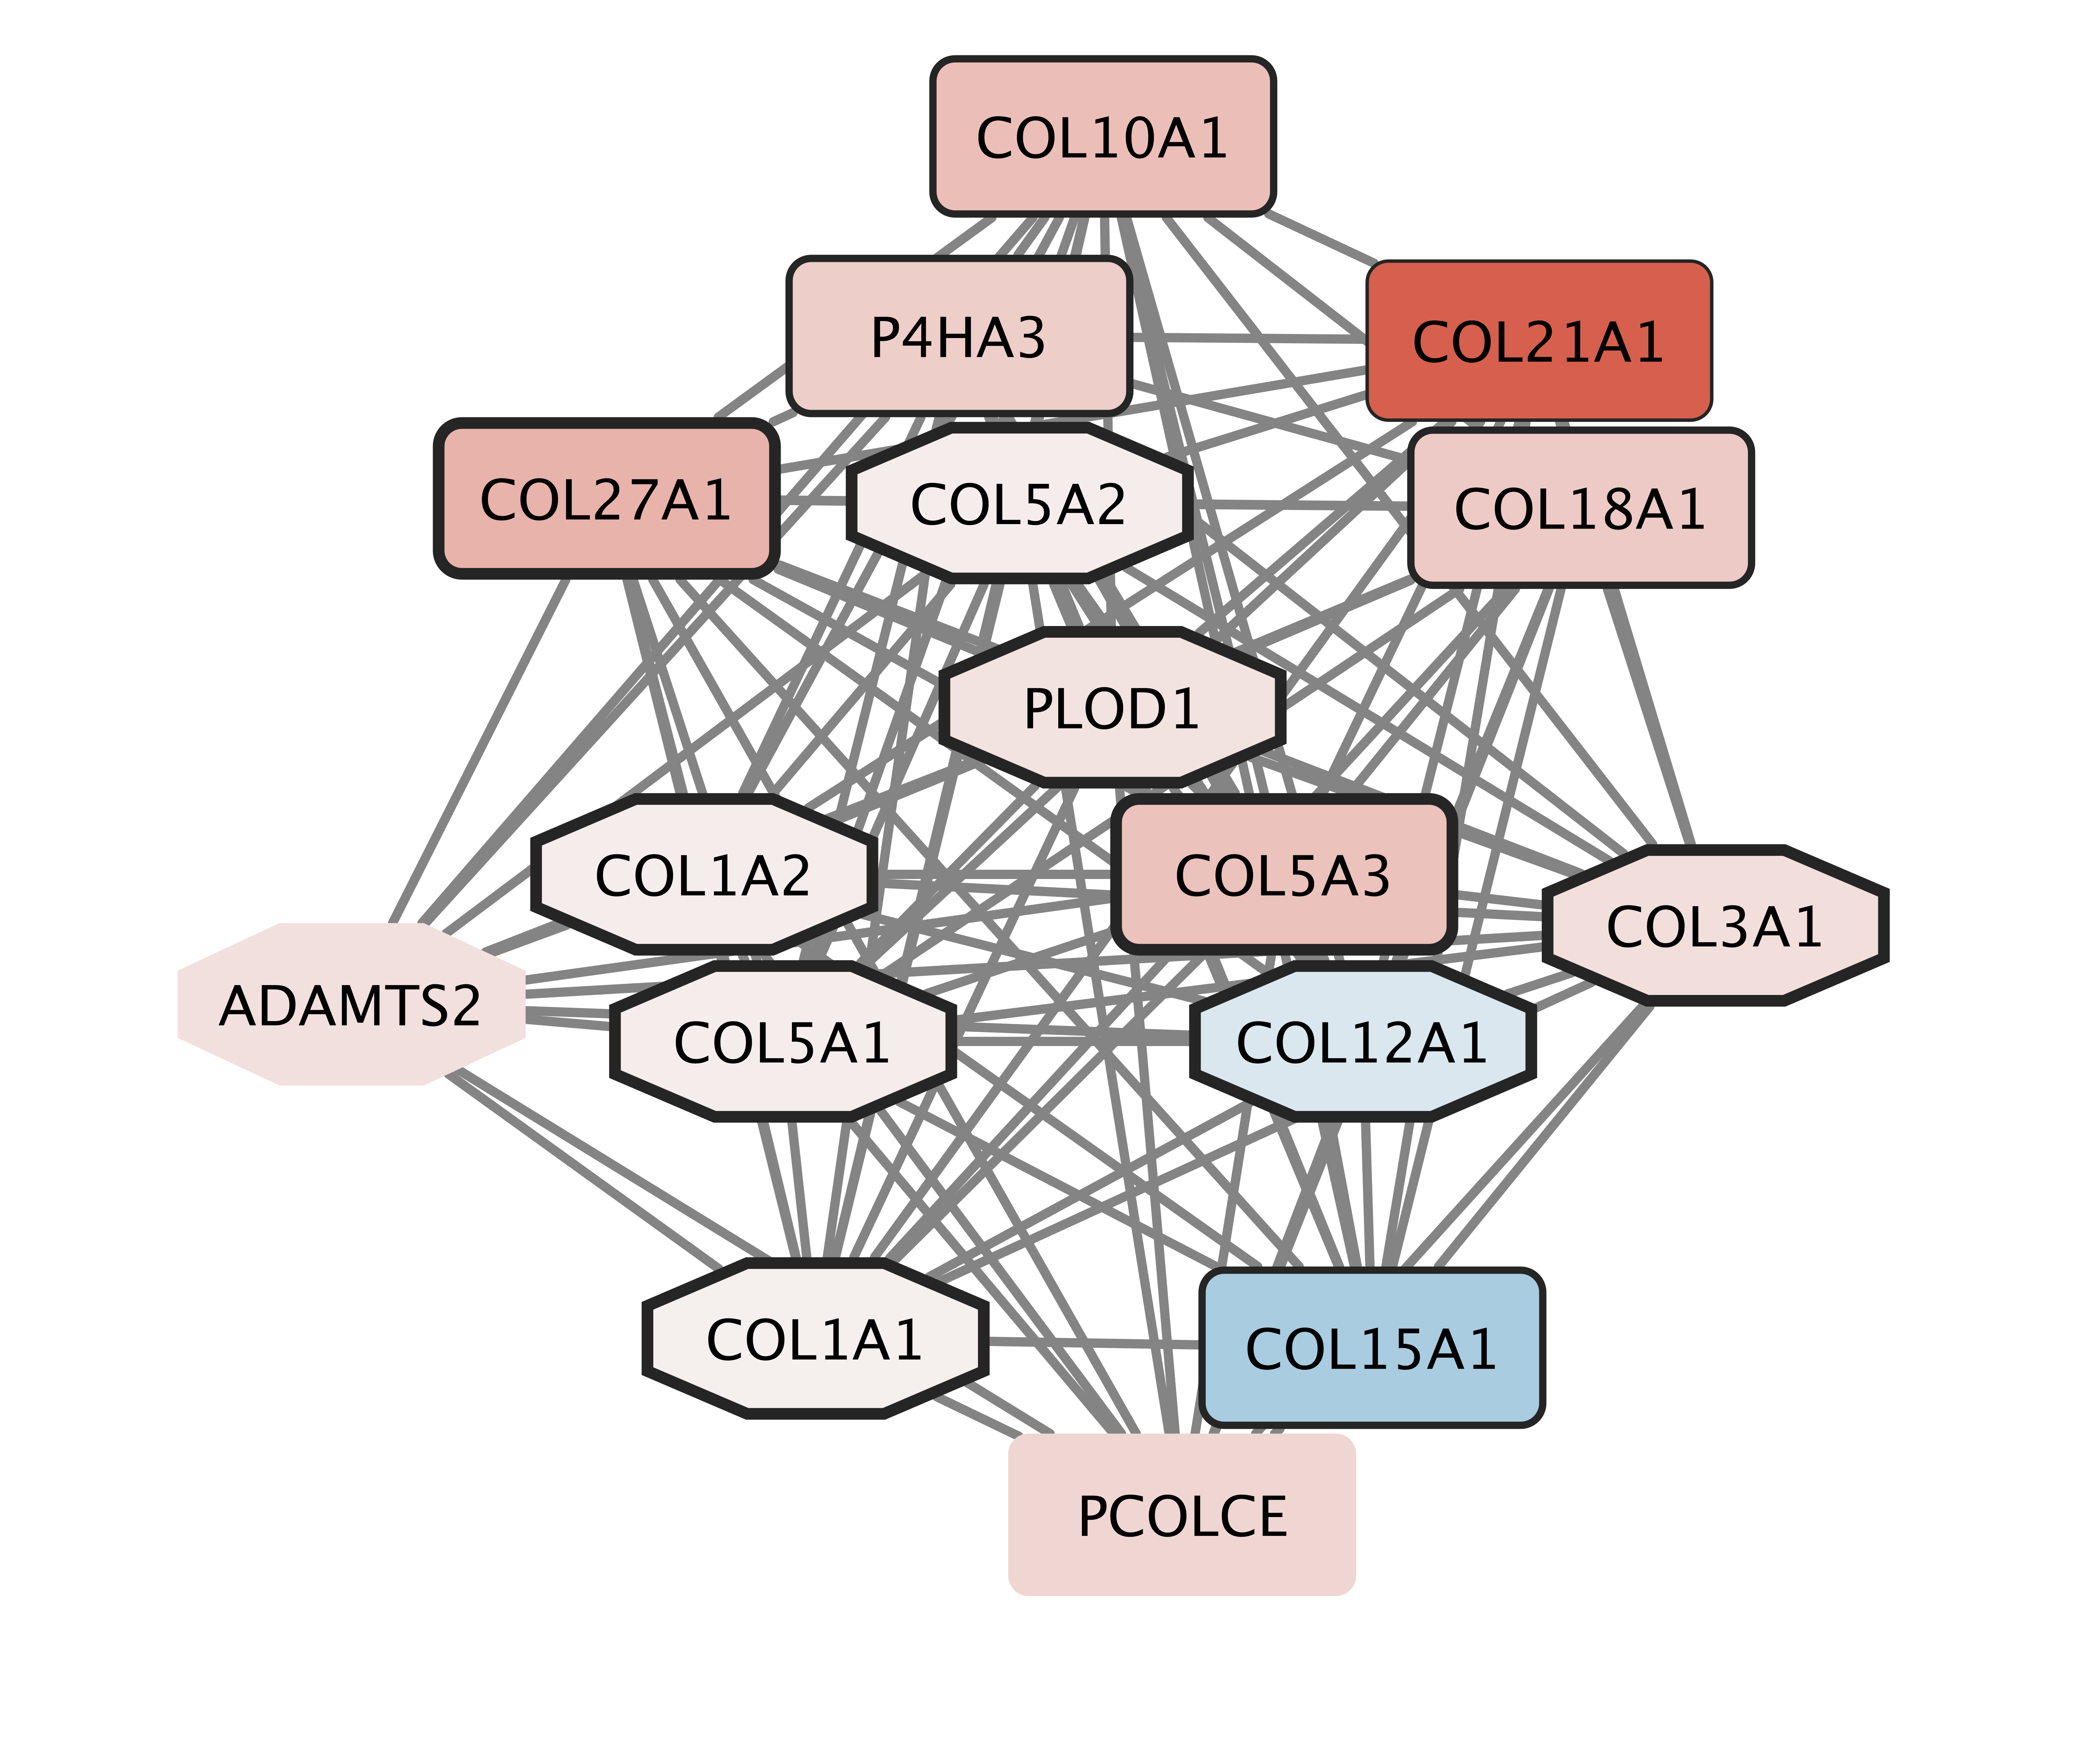
\includegraphics[width=0.7\textwidth]{fig/MCODE-cluster3.png}
	\caption[MCODE cluster 3]{\centering The MCODE cluster contains many genes known to cause other types of EDS. [TODO: add legend for shape, border and colour]}
	\label{fig:mcode3}
\end{figure}

GO-Enrichment testing overrepresentation of molecular functions of the cluster returns extracellular matrix in two terms, GO:0005201 and GO:0030020 with the second one being a subterm of the first. The first describes the action of a molecule that contributes to the structural integrity of the extracellular matrix, the second is a constituent of the extracellular matrix that enables the matrix to resist longitudinal stress. Both GO-terms contain the same EDS genes and seven respectively six other genes with PCOLE being the only gene not present in the GO subterm. These genes are investigated in more detail in terms of their centrality, differential expression and what is known about them. COL27A1, a fibrillar collagen gene has a central position in the cluster and relatively strong differential expression. The same applies for COL5A3, another gene related to collagen. The gene COL21A1 is very strongly differentially expressed, as mentioned before. It encodes the alpha chain of XXI collagen, which maintains the integrety of ECM and is a paralog to COL5A1, a known EDS gene \cite{COL21A1}.

To find connections to ECM in the enrichment analysis is consistent with findings of similar research \cite{Ritelli2022}. [Todo: there was other ressearch, find] The affection of ECM with particular disorganization of collagen and fibrocencting was found in hEDS and two other EDS types \cite{Chiarelli2018}. [TODO: point out what my new findings are, COL21A1 etc]

\paragraph{Up-regulated MCODE cluster}

The two larger, up-regulated MCODE clusters show no over-representation in ECM-terms, as is shown in figure \ref{fig:mcode-cluster-mf}. It is noticable, that the enrichment of the first cluster shows, that not many genes are part of the enriched terms. For the second cluster, the gene ratio is much higher, with up to around 80\,\% of the genes being involved in the second tow terms. Therefore the enrichment of the first cluster does not provide much insight in terms of molecular function in hEDS patients.

 \begin{figure}[htb]
 	\centering
 	\caption*{\textbf{Molecular function enrichment for the two larger up-regulated clusters}}
		\begin{subfigure}{.49\textwidth}
			\centering
 			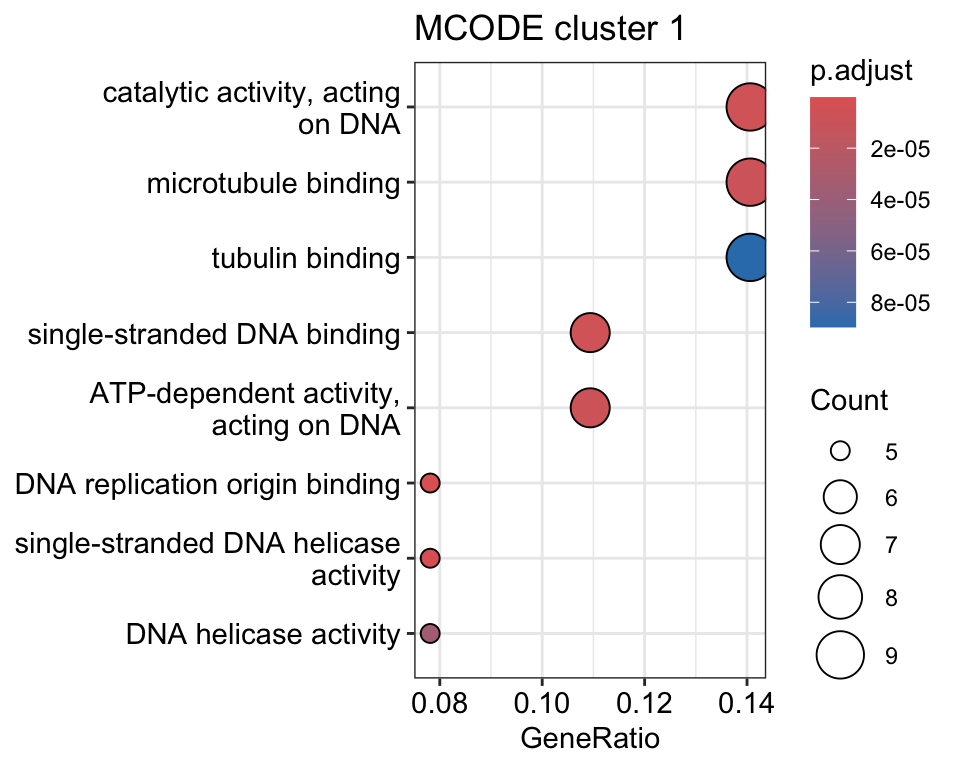
\includegraphics[width=\textwidth]{fig/mf-mcode-cluster1}
 			\caption{First MCODE cluster}
 		\end{subfigure}
    	\begin{subfigure}{.49\textwidth}
    		\centering
 			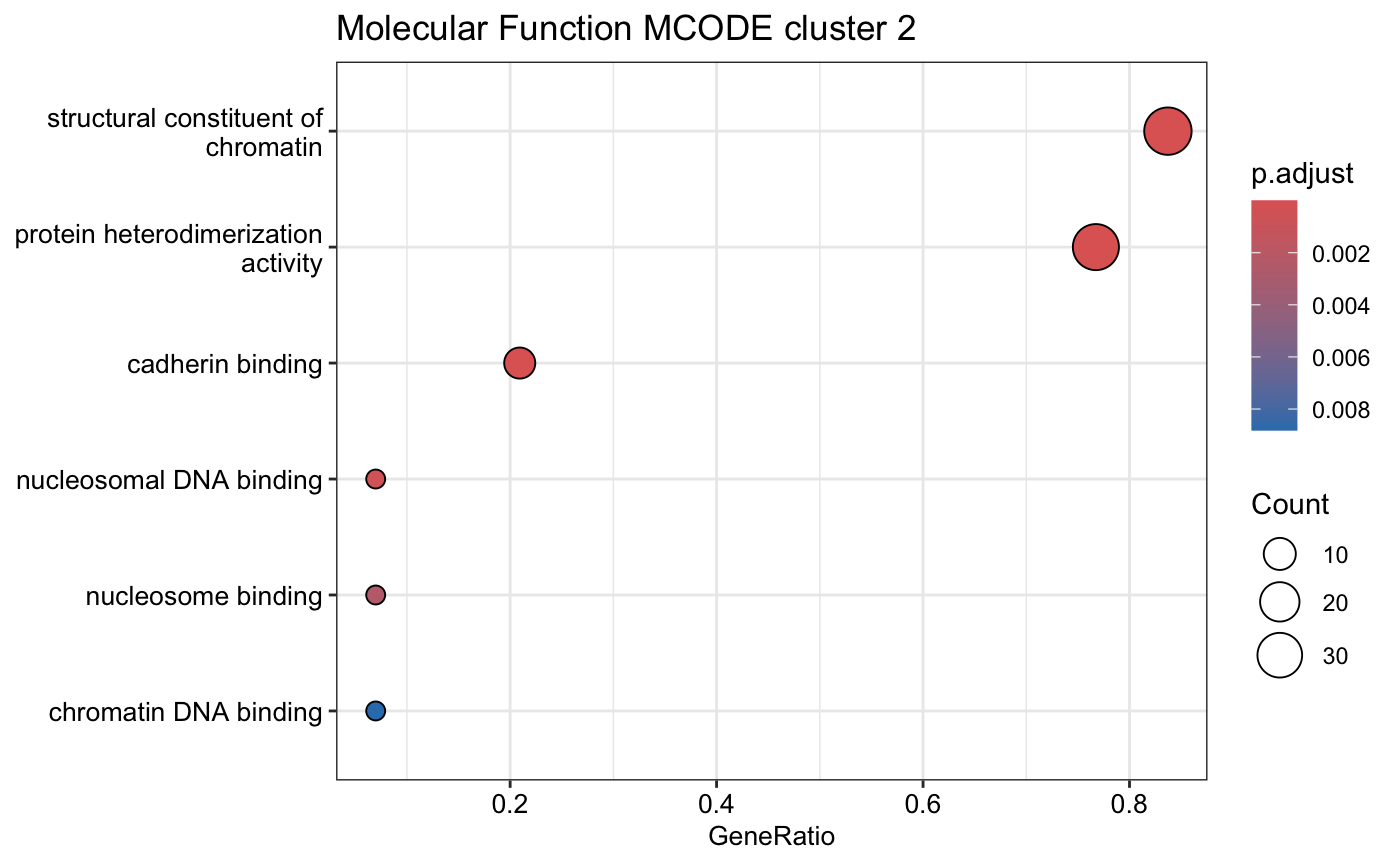
\includegraphics[width=\textwidth]{fig/mf-mcode-cluster2.png}
 			\caption{Second MCODE cluster}
 		\end{subfigure}
 	\caption{The results of the GO-enrichment for molecular function of the two up-regulated, larger MCODE clusters}
 	\label{fig:mcode-cluster-mf}
 \end{figure}

On the other hand, the up-regulation seen in the second cluster for the GO-term GO:0030527, the structural constituent of chromatin is interesting, because earlier research found down-regulated genes involved in processes related to chromatin in vEDS \cite{Chiarelli2018}.


\subsubsection{Community Clustering}

Community Clustering results in six clusters with more than 15 genes. Three of them are very small and loosely connected clusters, containing 18 to 29 genes and approximately the same amount of connections as genes. Since clusters of less than 20 genes are not large enough for analysis of biological processes, smaller clusters are ommited from the analysis. Additionally there are two medium-sized highly connected clusters with respectively 76 genes and 100 connections and 105 genes and 2330 connectinos and one very large cluster with 363 gens and 1661 connections. Especially the medium-sized clusters are highly interconnected and contain mostly up-regulated genes.

\paragraph{Largest Community Cluster}

The largest cluster contains a mix of up-regulated and down-regulated genes and also includes all 21 genes known to cause other EDS types. Furthermore, it contains all of the genes being part of the GO-term for the ECM found in the over-representation for molecular functions of the MCODE cluster containing the EDS genes. The molecular cluster showing enrichment towards the chromatin part is not a part of this community cluster.

Heat Diffusion 

\begin{itemize}
	\item 60 genes with heat $> 0.1$
	\item "hot genes" intersect with mcode cluster with eds genes: "COL27A1" "COL21A1" "COL10A1" "PCOLCE"  "COL18A1" "COL15A1" "COL5A3", "P4HA3", many of those are also the genes included in the ECM go-term
	\item expected since they are in the same cluster
	\item which other genes are also "hot"S
\end{itemize}





% all chromatin genes in Community cluster 5